\section{Results}
\label{sec:results}

\subsection{Campaign Completion}

All \val{campaign_runs_total} planned runs completed across \val{campaign_cells} balanced
cells. No run was lost to telemetry failure, no gateway was faulted, and every recovery time
was observed. %[id:campaign_runs_failed] %[id:campaign_gateway_runs] %[id:campaign_runs_censored]
Tables~\ref{tab:tbl_ieee_predictors_sn} and~\ref{tab:tbl_ieee_predictors_hr} list the graph
predictors and the measured outcomes of every analysed service.

\begin{table*}[!t]
\centering
\caption{Social Network: graph predictors and measured service medians for each analysed service}
\label{tab:tbl_ieee_predictors_sn}
\scriptsize
\setlength{\tabcolsep}{3pt}
\resizebox{\textwidth}{!}{%
\begin{tabular}{lrrrrrrrrrrrrr}
\toprule
\textbf{Service} & \textbf{Ancestors} & \textbf{Descendants} & \textbf{In-degree} & \textbf{Out-degree} & \textbf{HC} & \textbf{Betweenness} & \textbf{Closeness} & \textbf{PageRank} & \textbf{Eigenvector} & \textbf{\makecell[lb]{Degraded\\ancestors\\(kill)}} & \textbf{\makecell[lb]{Degraded\\ancestors\\(latency)}} & \textbf{\makecell[lb]{\textit{T}\textsubscript{rec}\\kill (s)}} & \textbf{\makecell[lb]{\textit{T}\textsubscript{rec}\\latency (s)}} \\
\midrule
post-storage-service & 4 & 0 & 3 & 0 & 0.109 & 0.000 & 0.291 & 0.157 & 0.000 & 4 & 4 & 15.3 & 15.4 \\
user-service & 4 & 0 & 2 & 0 & 0.073 & 0.000 & 0.242 & 0.145 & 0.000 & 2 & 2 & 14.5 & 14.8 \\
social-graph-service & 3 & 1 & 2 & 1 & 0.081 & 0.014 & 0.205 & 0.098 & 0.000 & 3 & 3 & 15.0 & 15.4 \\
url-shorten-service & 3 & 0 & 1 & 0 & 0.036 & 0.000 & 0.136 & 0.080 & 0.000 & 3 & 3 & 16.1 & 15.2 \\
user-mention-service & 3 & 0 & 1 & 0 & 0.036 & 0.000 & 0.136 & 0.080 & 0.000 & 3 & 3 & 14.5 & 14.4 \\
home-timeline-service & 2 & 3 & 2 & 2 & 0.096 & 0.012 & 0.182 & 0.074 & 0.000 & 2 & 2 & 15.4 & 15.6 \\
media-service & 2 & 0 & 1 & 0 & 0.036 & 0.000 & 0.121 & 0.061 & 0.000 & 2 & 2 & 16.1 & 14.8 \\
text-service & 2 & 2 & 1 & 2 & 0.064 & 0.036 & 0.121 & 0.061 & 0.000 & 2 & 2 & 15.3 & 14.4 \\
unique-id-service & 2 & 0 & 1 & 0 & 0.036 & 0.000 & 0.121 & 0.061 & 0.000 & 2 & 2 & 14.2 & 14.6 \\
user-timeline-service & 2 & 1 & 2 & 1 & 0.079 & 0.003 & 0.182 & 0.066 & 0.000 & 2 & 2 & 15.7 & 14.9 \\
compose-post-service & 1 & 10 & 1 & 7 & 0.302 & 0.053 & 0.091 & 0.062 & 0.000 & 1 & 1 & 15.6 & 15.6 \\
\bottomrule
\end{tabular}}
\end{table*}

\begin{table*}[!t]
\centering
\caption{Hotel Reservation: graph predictors and measured service medians for each analysed service}
\label{tab:tbl_ieee_predictors_hr}
\scriptsize
\setlength{\tabcolsep}{3pt}
\resizebox{\textwidth}{!}{%
\begin{tabular}{lrrrrrrrrrrrrr}
\toprule
\textbf{Service} & \textbf{Ancestors} & \textbf{Descendants} & \textbf{In-degree} & \textbf{Out-degree} & \textbf{HC} & \textbf{Betweenness} & \textbf{Closeness} & \textbf{PageRank} & \textbf{Eigenvector} & \textbf{\makecell[lb]{Degraded\\ancestors\\(kill)}} & \textbf{\makecell[lb]{Degraded\\ancestors\\(latency)}} & \textbf{\makecell[lb]{\textit{T}\textsubscript{rec}\\kill (s)}} & \textbf{\makecell[lb]{\textit{T}\textsubscript{rec}\\latency (s)}} \\
\midrule
geo & 2 & 0 & 1 & 0 & 0.057 & 0.000 & 0.190 & 0.152 & 0.707 & 2 & 2 & 22.0 & 17.7 \\
rate & 2 & 0 & 1 & 0 & 0.057 & 0.000 & 0.190 & 0.152 & 0.707 & 2 & 2 & 20.9 & 16.9 \\
profile & 1 & 0 & 1 & 0 & 0.057 & 0.000 & 0.143 & 0.124 & 0.002 & 1 & 1 & 27.0 & 18.7 \\
recommendation & 1 & 0 & 1 & 0 & 0.057 & 0.000 & 0.143 & 0.107 & 0.002 & 1 & 1 & 22.6 & 25.4 \\
reservation & 1 & 0 & 1 & 0 & 0.057 & 0.000 & 0.143 & 0.127 & 0.002 & 1 & 1 & 19.3 & 16.6 \\
search & 1 & 2 & 1 & 2 & 0.112 & 0.048 & 0.143 & 0.119 & 0.002 & 1 & 1 & 22.3 & 24.7 \\
user & 1 & 0 & 1 & 0 & 0.057 & 0.000 & 0.143 & 0.119 & 0.002 & 1 & 1 & 19.7 & 13.6 \\
\bottomrule
\end{tabular}}
\end{table*}


\subsection{The Confirmatory Test of H1}
\label{sec:res-h1}

On Social Network under kill faults, the caller count $X$ and the number of degraded callers
$Y$ correlate at $\rho = \val{primary_rho}$ across \val{primary_n_services} services, with a
bias-corrected and accelerated bootstrap interval from \val{primary_ci_lo} to
\val{primary_ci_hi}. The uncorrected p-value from \val{primary_n_permutations} random
permutations is \val{primary_p_locked}. After Benjamini-Hochberg correction across the
\val{conf_family_size} tests of the confirmatory family, the adjusted p-value is
\val{primary_p_bh_locked}. Exact enumeration, run after the results were known (Deviation 9),
gives \val{primary_p_exact} uncorrected and \val{primary_p_bh_exact} adjusted, and the verdict
does not change.\footnote{The locked Monte Carlo values remain the preregistered result.}
%[id:primary_significant_exact] %[id:primary_ci_method]

Not one of the \val{conf_family_size} confirmatory tests reaches significance at
$q = \val{fdr_q}$.
%[id:conf_family_significant]
The primary test has the smallest uncorrected p-value in the family, %[id:conf_best_raw_p] %[id:conf_best_predictor]
and its adjusted value is about \val{primary_p_bh_over_q} times the threshold.
Table~\ref{tab:tbl_ieee_primary} gives the primary test for each family and application, and
Table~\ref{tab:tbl_ieee_families} summarises both families. H1 is not confirmed. The point
estimate is large and positive, the correction fixed in advance rejects it, and the interval
runs from no association to a perfect one.

\begin{table*}[!t]
\centering
\caption{Test of H1, caller count $X$ against degraded callers $Y$, in each family and application}
\label{tab:tbl_ieee_primary}
\scriptsize
\setlength{\tabcolsep}{3pt}

\begin{tabular}{lllrrllrp{2.3cm}rlp{2.0cm}}
\toprule
\textbf{Family} & \textbf{Fault} & \textbf{Application} & \textbf{Services} & \textbf{$\rho$} & \textbf{95\% CI} & \textbf{CI method} & \textbf{p (raw)} & \textbf{p method} & \textbf{p (BH)} & \textbf{Significant} & \textbf{Note} \\
\midrule
confirmatory & kill & Social Network & 11 & 0.785 & 0.000 to 1.000 & BCa & 0.0080 & Monte Carlo, 10,000 permutations & 0.3451 & no &  \\
confirmatory & kill & Hotel Reservation & 7 & 1.000 & 1.000 to 1.000 & percentile & 0.0476 & exact, 5,040 permutations & 0.3451 & no & saturated; directional only \\
replication & latency & Social Network & 11 & 0.785 & 0.000 to 1.000 & BCa & 0.0076 & Monte Carlo, 10,000 permutations & 0.1848 & no &  \\
replication & latency & Hotel Reservation & 7 & 1.000 & 1.000 to 1.000 & percentile & 0.0476 & exact, 5,040 permutations & 0.2328 & no & saturated; directional only \\
\bottomrule
\end{tabular}
\end{table*}

\begin{table*}[!t]
\centering
\caption{Family sizes and the number of tests that survive Benjamini-Hochberg correction}
\label{tab:tbl_ieee_families}
\footnotesize
\setlength{\tabcolsep}{3pt}

\begin{tabular}{llrrrrrp{5.0cm}}
\toprule
\textbf{Family} & \textbf{Fault} & \textbf{Tests} & \textbf{\makecell[lb]{Tests with\\defined p}} & \textbf{\makecell[lb]{Significant\\after BH}} & \textbf{\makecell[lb]{Smallest p\\(raw)}} & \textbf{Its p (BH)} & \textbf{Test with the smallest p} \\
\midrule
confirmatory & kill & 44 & 44 & 0 & 0.0080 & 0.3451 & Social Network, caller count \textit{X} against \textit{Y} \\
replication & latency & 44 & 44 & 0 & 0.0076 & 0.1848 & Social Network, caller count \textit{X} against \textit{Y} \\
\bottomrule
\end{tabular}
\end{table*}


Two features of the data qualify the estimate further, and they matter more than its p-value.
The first is saturation. Since $Y$ counts degraded callers and $X$ counts callers, $Y$ can never
exceed $X$, and if every service's measured count equalled its graph count the correlation
would be one by construction and would test nothing. On Hotel Reservation that is what
happened: each service's measured outcome matched its predictor in every run, under both fault
types. %[id:saturation_hr_kill_run] %[id:saturation_hr_kill_service] %[id:saturation_hr_latency_run]
Hotel Reservation is therefore tautological at the unit of analysis,
%[id:saturation_hr_kill_tautological]
and every Hotel Reservation result is reported as directional only.

Social Network is not fully saturated. Its run-level saturation under kill faults is
\val{saturation_sn_kill_run}, which is why $\rho$ falls short of one. Fig.~\ref{fig:primary}
shows the pattern: ten of the eleven services lie exactly on the line $y = x$.
%[id:saturation_sn_kill_service]
One departs from it. User-service has \val{userservice_ancestor_count} graph ancestors and
registered \val{userservice_measured} degraded ancestors in all \val{userservice_runs_departing}
of its kill repetitions. The empirical content of the Social Network correlation, as distinct
from its definitional content, rests on that one service. A leave-one-out recomputation,
designed after the confirmatory result was known and carrying no inferential weight, withholds
one service at a time (Fig.~\ref{fig:loo}). The correlation then ranges from
\val{loo_rho_min} to \val{loo_rho_max}, and the value of \val{loo_userservice_rho} comes from
withholding user-service.

\begin{figure*}[!t]
\centering
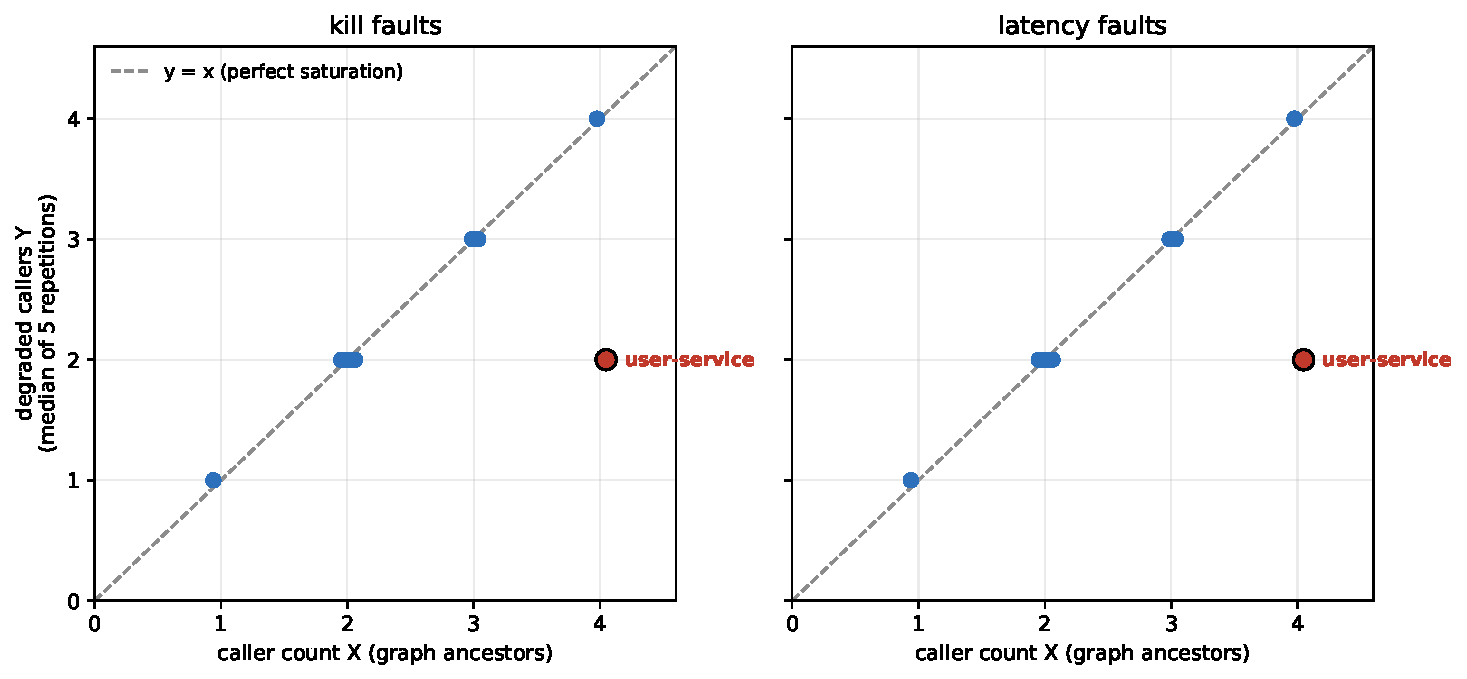
\includegraphics[width=0.78\textwidth]{generated/figures/fig_primary_sn.pdf}
\caption{Caller count $X$ against the measured number of degraded callers $Y$ for each Social
Network service under kill and latency faults. Points on the dashed line $y = x$ are
saturated; the labelled service departs from it.}
\label{fig:primary}
\end{figure*}

\begin{figure*}[!t]
\centering
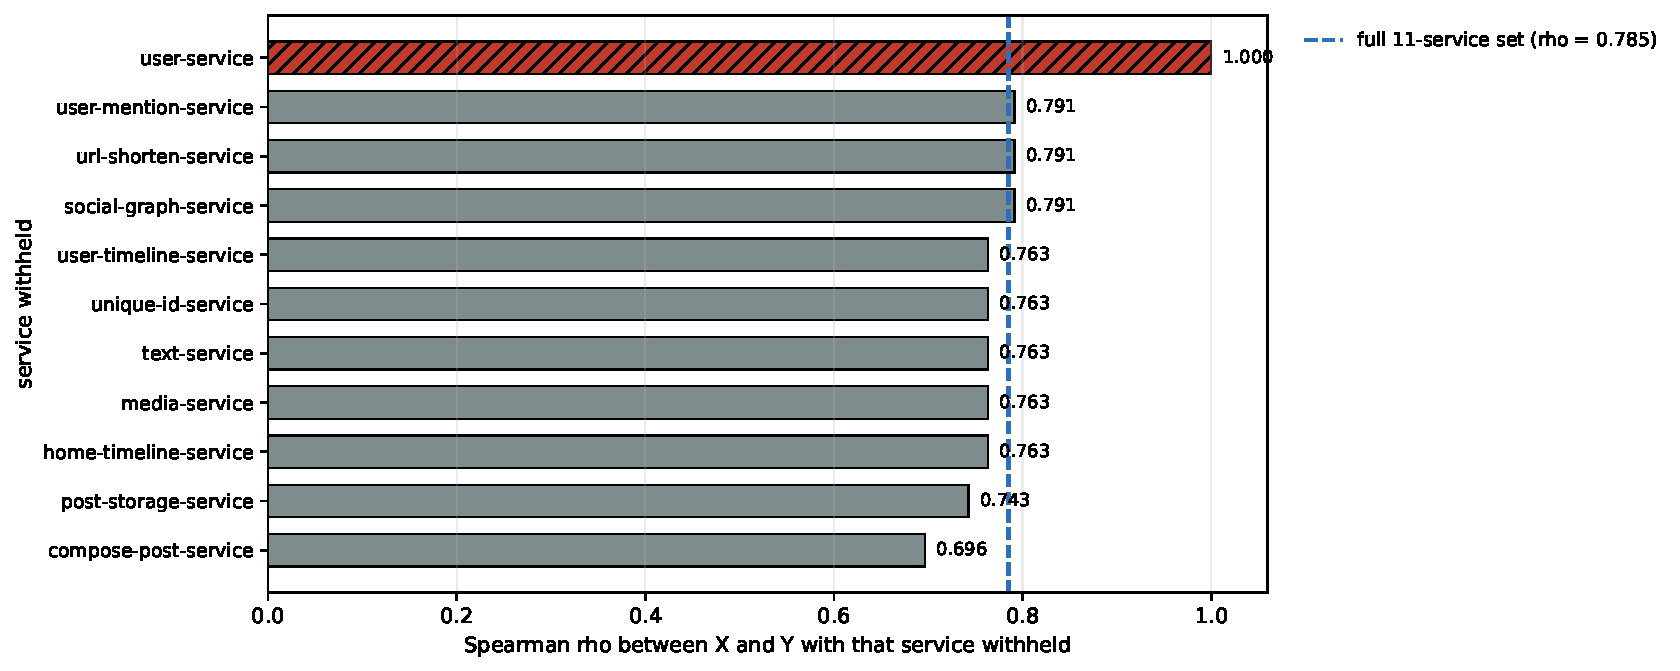
\includegraphics[width=0.78\textwidth]{generated/figures/fig_leave_one_out.pdf}
\caption{Post hoc leave-one-out check: Spearman's $\rho$ between $X$ and $Y$ on Social Network
under kill faults, recomputed with each service withheld.}
\label{fig:loo}
\end{figure*}

\subsection{The Hybrid Metric and H2}
\label{sec:res-h2}

The hybrid metric combines inbound centrality with a fan-out-scaled outbound term, on the
premise that a service calling many others matters because its failure breaks many downstream
links. H2 expected that premise to point the wrong way. Table~\ref{tab:tbl_ieee_h2} gives all
\val{h1b_cells} application and fault combinations. They are not independent: the outcome
vectors coincide across fault types, %[id:replication_primary_identical]
so the four cells hold \val{h1b_distinct_comparisons} distinct comparisons, one per application.

\begin{table*}[!t]
\centering
\caption{Test of H2, the hybrid metric HC against degraded callers $Y$, in all four application and fault cells}
\label{tab:tbl_ieee_h2}
\footnotesize
\setlength{\tabcolsep}{3pt}

\begin{tabular}{lllrrlrrlp{2.6cm}}
\toprule
\textbf{Family} & \textbf{Fault} & \textbf{Application} & \textbf{Services} & \textbf{$\rho$} & \textbf{95\% CI} & \textbf{p (raw)} & \textbf{p (BH)} & \textbf{$\rho$ $\leq$ 0} & \textbf{Distinguishable from zero after BH} \\
\midrule
confirmatory & kill & Social Network & 11 & \textminus{}0.144 & \textminus{}0.810 to 0.698 & 0.6688 & 0.9925 & yes & no \\
confirmatory & kill & Hotel Reservation & 7 & \textminus{}0.258 & \textminus{}0.730 to \textminus{}0.167 & 1.0000 & 1.0000 & yes & no \\
replication & latency & Social Network & 11 & \textminus{}0.144 & \textminus{}0.805 to 0.713 & 0.6656 & 0.9152 & yes & no \\
replication & latency & Hotel Reservation & 7 & \textminus{}0.258 & \textminus{}0.750 to \textminus{}0.167 & 1.0000 & 1.0000 & yes & no \\
\bottomrule
\end{tabular}
\end{table*}


The correlation between the hybrid metric and $Y$ is negative in every cell,
%[id:h1b_all_negative]
$\rho = \val{h1b_sn_kill_rho}$ on Social Network under both kill and latency faults
%[id:h1b_sn_latency_rho]
and $\rho = \val{h1b_hr_kill_rho}$ on Hotel Reservation. %[id:h1b_hr_latency_rho]
After correction no cell can be told apart from zero. %[id:h1b_any_distinguishable]
The adjusted p-values are \val{h1b_sn_kill_bh_p} and \val{h1b_sn_latency_bh_p} on Social
Network and \val{h1b_hr_kill_bh_p} on Hotel Reservation, %[id:h1b_hr_latency_bh_p]
and the Social Network interval runs from \val{h1b_sn_kill_ci_lo} to \val{h1b_sn_kill_ci_hi}.
The direction H2 states appears every time, but its size cannot be separated from zero, so no
negative relationship is claimed. What the data show is an absence of support for the fan-out
premise.

\subsection{The Motivating Case}

The metric was first motivated by compose-post-service, which calls
\val{composepost_out_degree} services directly and has \val{composepost_descendants}
transitive descendants. On the strength of that fan-out, the hybrid metric ranks it first of the
\val{composepost_set_size} analysed services, %[id:composepost_rank_hybrid]
with a score of \val{composepost_hybrid}. By transitive callers it ranks last, having a single
graph ancestor. %[id:composepost_rank_ancestor_count] %[id:composepost_ancestor_count]
Fig.~\ref{fig:rank} shows the full rank inversion.

\begin{figure}[!t]
\centering
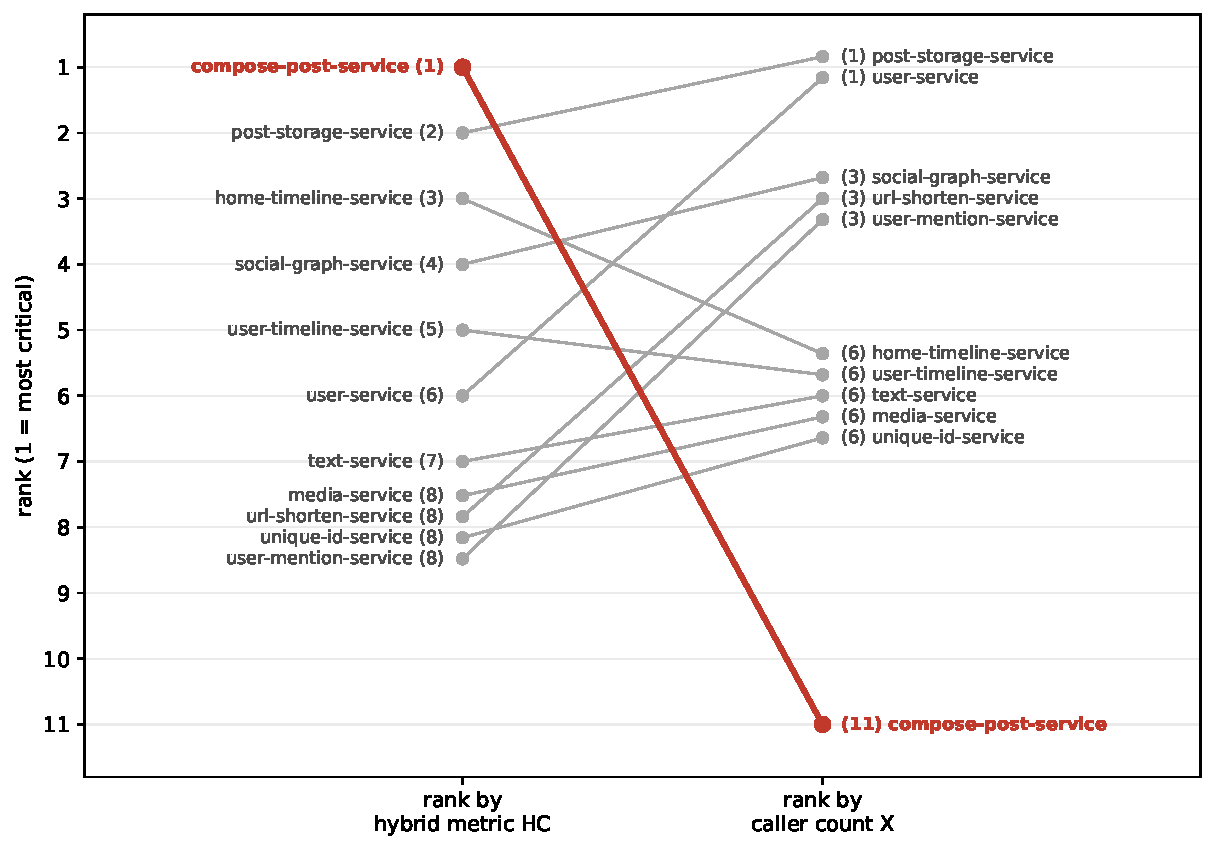
\includegraphics[width=\columnwidth]{generated/figures/fig_rank_inversion.pdf}
\caption{Rank of the eleven Social Network services by the hybrid metric HC and by caller
count $X$, with compose-post-service highlighted.}
\label{fig:rank}
\end{figure}

Measurement agrees with the caller-based ranking. Faulting compose-post-service left exactly
one degraded ancestor in each of its \val{composepost_kill_reps} kill repetitions,
%[id:composepost_kill_min] %[id:composepost_kill_max]
and the latency runs gave the same result. %[id:composepost_latency_min] %[id:composepost_latency_max]
A post hoc breakdown shows that in all \val{composepost_runs_total} runs that ancestor was
nginx-web-server, the gateway. %[id:composepost_runs_only_gateway_ancestor]
On the preregistered outcome, the service the original metric rates most critical is the lowest
in its application. The outcome counts degraded services, though, and does not measure requests
or functionality lost, and this is a single worked case: the test across all eleven services,
which could have generalised it, is the null result of Section~\ref{sec:res-h1}.

\subsection{Replication under a Second Fault Type}

The replication family repeats all \val{repl_family_size} tests on latency faults. Again no test
is significant after correction. %[id:repl_family_significant]
The smallest uncorrected p-value is \val{repl_best_raw_p}, with an adjusted value of
\val{repl_best_bh_p}. The agreement carries a caveat. Under kill and latency faults the service
medians of $Y$ are identical in both applications, %[id:replication_primary_identical]
and at run level \val{fault_invariant_services_all} of the
\val{fault_invariant_services_all_total} services show the same five per-run counts under both
fault types. On the primary outcome the latency family therefore repeats the kill family's
correlations on the same values and adds no independent evidence about H1.

Read on its own, this says that which services degrade when a service fails hardly depends on
how it fails: a process that disappears and a process that slows down reach the same
neighbours. Recovery differs. The correlation between median recovery times under kill and
under latency faults is \val{trec_rho_between_faults_sn} on Social Network and
\val{trec_rho_between_faults_hr} on Hotel Reservation, so for recovery time the second fault
type does add information.

\subsection{Direction of Propagation}
\label{sec:res-direction}

Across the campaign, degradation travelled to callers and not to callees. No descendant of the
faulted service degraded in \val{descendant_affected_runs_zero} of \val{campaign_runs_total}
runs, %[id:descendant_affected_runs_zero_pct]
and at the unit of analysis, the median over a service's repetitions, the count is zero for
every service under both fault types. %[id:descendant_affected_count_constant_at] %[id:descendant_affected_count_distinct_values]
The single exception, a kill repetition of compose-post-service on Social Network, recorded
\val{descendant_affected_max_in_any_run} degraded descendants.
%[id:descendant_affected_runs_nonzero] %[id:descendant_affected_exception_run]
Services unrelated to the faulted one behave the same way, with
\val{unrelated_affected_runs_zero} of \val{campaign_runs_total} runs at zero and one exception.
%[id:unrelated_affected_exception_run]

This is the firmest structural result of the study, and it cannot be written as a correlation.
Neither outcome varies between services, so \val{expl_undefined} of the \val{expl_attempted}
exploratory tests attempted have no defined value. A constant outcome gives no correlation at
all, which is different from a weak one. These tests are reported as undefined, with the
reason, in the same way as the \val{degenerate_pairs} degenerate predictors, and are not
entered as zeros.

\subsection{Exploratory Findings}

Of the \val{expl_testable} testable exploratory tests, \val{expl_significant} survive correction
within that family. Both concern the size of latency inflation under latency faults on Social
Network: the change in p95 correlates with the hybrid metric at
$\rho = \val{expl_sig_hybrid_criticality_rho}$ and with plain degree at
$\rho = \val{expl_sig_degree_rho}$, both with an adjusted p of
\val{expl_sig_hybrid_criticality_bh_p}. %[id:expl_sig_degree_bh_p]
These results carry no confirmatory weight, and their outcome is not the one H2 concerns. How
much latency inflates differs from how many callers degrade, and plain degree does at least as
well as the hybrid metric on it, which gives no reason to prefer the fan-out correction.

\subsection{What the Design Could Have Detected}
\label{sec:res-power}

Table~\ref{tab:tbl_ieee_power} reproduces the preregistered power analysis on the realised
analysis sets. Both sets have the registered size and the registered number of distinct
predictor values, and the ceiling correlations come out exactly as preregistered.
%[id:power_sn_n_matches] %[id:power_hr_n_matches] %[id:power_sn_levels_match] %[id:power_hr_levels_match] %[id:power_sn_ceiling_matches] %[id:power_hr_ceiling_matches]
The caller count takes only \val{power_sn_levels} distinct values across the
\val{power_sn_n} Social Network services and \val{power_hr_levels} across the \val{power_hr_n}
Hotel Reservation services. For an outcome without ties, these ties cap the attainable
correlation at \val{power_sn_ceiling} and \val{power_hr_ceiling}.

\begin{table}[!t]
\centering
\caption{Preregistered power analysis reproduced on the realised analysis sets; permutation p-values from 10000 random permutations (Social Network) and exact enumeration of 5040 permutations (Hotel Reservation)}
\label{tab:tbl_ieee_power}
\footnotesize
\setlength{\tabcolsep}{3pt}

\begin{tabular}{p{3.9cm}p{2.0cm}p{1.9cm}}
\toprule
\textbf{Quantity} & \textbf{Social Network} & \textbf{Hotel Reservation} \\
\midrule
Services, realised / preregistered & 11 / 11 & 7 / 7 \\
Distinct \textit{X} values, realised / preregistered & 4 / 4 & 2 / 2 \\
\textit{X} values & 1, 2, 2, 2, 2, 2, 3, 3, 3, 4, 4 & 1, 1, 1, 1, 1, 2, 2 \\
Ceiling $\rho$, outcome without ties, realised / preregistered & 0.941 / 0.941 & 0.791 / 0.791 \\
Ceiling p, outcome without ties, permutation & 0.0002 & 0.0952 \\
Ceiling p, outcome without ties, asymptotic (not for inference) & $<$0.0001 & 0.0343 \\
Ceiling $\rho$, outcome tied like \textit{X} & 1.000 & 1.000 \\
Ceiling p, outcome tied like \textit{X}, permutation & 0.0001 & 0.0476 \\
p quoted in the preregistration &  & 0.034 \\
\bottomrule
\end{tabular}
\end{table}


For Hotel Reservation the limit is severe. An outcome without ties can reach at best
$\rho = \val{power_hr_ceiling}$, with an exact permutation p of \val{power_hr_ceiling_p}, above
the conventional threshold before any correction. The preregistration quoted
\val{power_hr_prereg_stated_p} for this ceiling, which is the asymptotic value; the exact value
the plan requires is the one above (Deviation 7). Only an outcome that repeats the predictor's
own ties can do better, reaching $\rho = \val{power_hr_tied_rho}$ with p =
\val{power_hr_tied_p}, and saturation produced exactly that outcome
(Table~\ref{tab:tbl_ieee_primary}). Hotel Reservation could therefore pass the nominal threshold
before correction only by restating its predictor, and after correction its primary test is
far from significant. That follows from its tie structure and its size, not from anything
measured.

\subsection{Recovery Time}
\label{sec:res-trec}

No run was censored, so under the preregistered rule the Spearman rank test is the primary test
for recovery time, and the Cox and log-rank models are secondary and uncorrected (Deviation 6).
Table~\ref{tab:tbl_ieee_trec} gives all three for both predictors. No recovery-time test is
significant after correction in either family. %[id:trec_conf_significant] %[id:trec_repl_significant]
The log-rank test is undefined for \val{trec_conf_logrank_undefined} of the
\val{trec_conf_tests} recovery-time tests in each family, %[id:trec_repl_logrank_undefined] %[id:trec_repl_tests]
among them $X$ on Hotel Reservation, where the predictor has fewer than two distinct terciles.
Supplementary file S2 gives the unrounded estimates.

\begin{table*}[!t]
\centering
\caption{Recovery time: Spearman's $\rho$ (primary, BH-corrected within each family) and Cox and log-rank tests (secondary, uncorrected). Hazard ratios are per one-unit increase of the predictor, fitted per run with service-clustered errors and per service; the hybrid metric spans less than one unit, so its hazard ratios extrapolate beyond the observed range. Log-rank is undefined where the predictor has fewer than two distinct terciles}
\label{tab:tbl_ieee_trec}
\scriptsize
\setlength{\tabcolsep}{3pt}
\resizebox{\textwidth}{!}{%
\begin{tabular}{lllrrrrrrrrrr}
\toprule
\textbf{Fault} & \textbf{Application} & \textbf{Predictor} & \textbf{$\rho$} & \textbf{p (raw)} & \textbf{p (BH)} & \textbf{\makecell[lb]{HR per\\unit, run}} & \textbf{95\% CI, run} & \textbf{p, run} & \textbf{\makecell[lb]{HR per\\unit,\\service}} & \textbf{\makecell[lb]{95\% CI,\\service}} & \textbf{p, service} & \textbf{Log-rank p} \\
\midrule
kill & Social Network & caller count \textit{X} & \textminus{}0.356 & 0.2807 & 0.9264 & 1.173 & 0.876 to 1.570 & 0.2836 & 1.479 & 0.688 to 3.181 & 0.3163 & 0.5154 \\
kill & Social Network & hybrid metric HC & 0.098 & 0.7699 & 0.9925 & 0.010 & 0.002 to 0.043 & $<$0.0001 & 1.408 & $5.49\times10^{-4}$ to $3.61\times10^{3}$ & 0.9319 & 0.2099 \\
kill & Hotel Reservation & caller count \textit{X} & \textminus{}0.158 & 0.8571 & 0.9925 & 1.522 & 1.067 to 2.171 & 0.0204 & 2.179 & 0.302 to 15.722 & 0.4399 & undefined \\
kill & Hotel Reservation & hybrid metric HC & 0.204 & 0.8571 & 0.9925 & 0.147 & $8.91\times10^{-4}$ to 24.134 & 0.4609 & not estimable & not estimable & not estimable & undefined \\
latency & Social Network & caller count \textit{X} & \textminus{}0.060 & 0.8647 & 1.0000 & 0.998 & 0.816 to 1.221 & 0.9859 & 1.184 & 0.627 to 2.236 & 0.6018 & 0.5561 \\
latency & Social Network & hybrid metric HC & 0.767 & 0.0084 & 0.1848 & 0.045 & 0.002 to 1.163 & 0.0616 & $2.49\times10^{-4}$ & $8.19\times10^{-10}$ to 75.493 & 0.1975 & 0.1099 \\
latency & Hotel Reservation & caller count \textit{X} & \textminus{}0.158 & 0.8571 & 1.0000 & 0.882 & 0.578 to 1.346 & 0.5609 & 2.179 & 0.302 to 15.722 & 0.4399 & undefined \\
latency & Hotel Reservation & hybrid metric HC & 0.408 & 0.5714 & 0.8111 & $6.26\times10^{-4}$ & $1.07\times10^{-6}$ to 0.368 & 0.0234 & not estimable & not estimable & not estimable & undefined \\
\bottomrule
\end{tabular}}
\par\smallskip\parbox{\linewidth}{\scriptsize Not estimable: the Cox fit did not converge or showed separation because the predictor takes few distinct values; raw estimates are in supplementary file S2.}
\end{table*}


\subsection{Post Hoc Weight Sensitivity}
\label{sec:res-weights}

The confirmatory results were already in hand when this analysis was designed, and it belongs
to no preregistered family. It asks how much the hybrid metric's association with the outcome
depends on its weights. The metric was recomputed for all \val{ws_triplets} weight triplets on
the preregistered grid, with step \val{ws_grid_step} and weights summing to one, using the same
code, the same service medians and the same permutation tests. Each set of
\val{ws_triplets} tests was corrected with the Benjamini-Hochberg procedure within that set. No
triplet was selected or adopted, and every other result in this paper uses the reported
weights. Table~\ref{tab:tbl_ieee_weights} and Fig.~\ref{fig:weights} give the full distribution.

\begin{table*}[!t]
\centering
\caption{Post hoc weight sensitivity of the hybrid metric over 231 weight triplets, with BH correction within each set of 231}
\label{tab:tbl_ieee_weights}
\scriptsize
\setlength{\tabcolsep}{3pt}

\begin{tabular}{lllrrrrrrrrr}
\toprule
\textbf{Application} & \textbf{Fault} & \textbf{Outcome} & \textbf{\makecell[lb]{Triplets\\with\\defined $\rho$}} & \textbf{$\rho$ min} & \textbf{$\rho$ median} & \textbf{$\rho$ max} & \textbf{$\rho$ $>$ 0} & \textbf{\makecell[lb]{p (raw) $<$\\0.05}} & \textbf{\makecell[lb]{Significant\\after BH}} & \textbf{\makecell[lb]{$\rho$ at\\0.4/0.4/0.2}} & \textbf{\makecell[lb]{p at\\0.4/0.4/0.2}} \\
\midrule
Social Network & kill & degraded callers \textit{Y} & 231 & \textminus{}0.544 & \textminus{}0.167 & 0.337 & 28 & 0 & 0 & \textminus{}0.144 & 0.6695 \\
Social Network & latency & degraded callers \textit{Y} & 231 & \textminus{}0.544 & \textminus{}0.167 & 0.337 & 28 & 0 & 0 & \textminus{}0.144 & 0.6695 \\
Hotel Reservation & kill & degraded callers \textit{Y} & 230 & \textminus{}0.258 & \textminus{}0.258 & \textminus{}0.258 & 0 & 0 & 0 & \textminus{}0.258 & 1.0000 \\
Hotel Reservation & latency & degraded callers \textit{Y} & 230 & \textminus{}0.258 & \textminus{}0.258 & \textminus{}0.258 & 0 & 0 & 0 & \textminus{}0.258 & 1.0000 \\
Social Network & kill & gateway error rate & 231 & 0.229 & 0.753 & 0.832 & 231 & 145 & 128 & 0.786 & 0.0064 \\
Hotel Reservation & kill & gateway error rate & 230 & \textminus{}0.204 & \textminus{}0.204 & \textminus{}0.204 & 0 & 0 & 0 & \textminus{}0.204 & 0.8571 \\
\bottomrule
\end{tabular}
\end{table*}


\begin{figure}[!t]
\centering
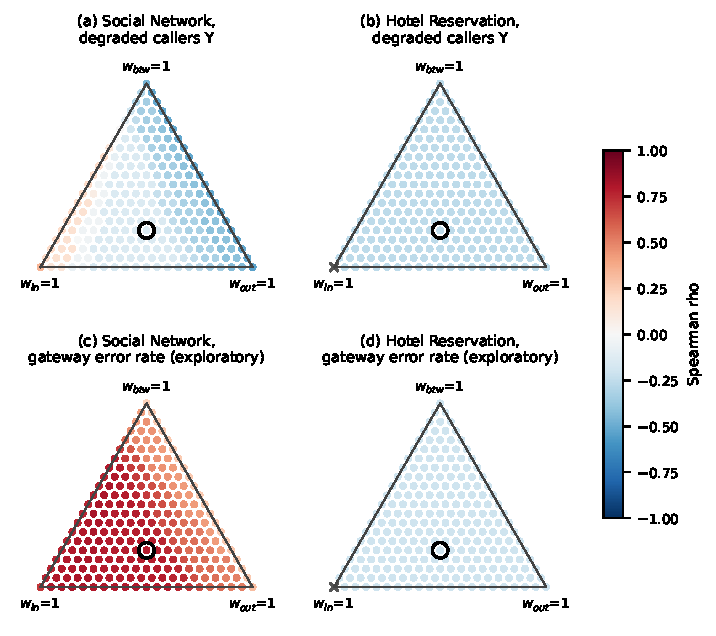
\includegraphics[width=\columnwidth]{generated/figures/fig_weight_sensitivity.pdf}
\caption{Post hoc weight sensitivity: Spearman's $\rho$ of the hybrid metric against degraded
callers (a, b) and the gateway error rate (c, d) for every weight triplet under kill faults;
latency faults give identical results for degraded callers. Circled: the reported weights;
cross: metric constant.}
\label{fig:weights}
\end{figure}

Against the number of degraded callers on Social Network, $\rho$ ranged from
\val{ws_sn_kill_anc_rho_min} to \val{ws_sn_kill_anc_rho_max}, with a median of
\val{ws_sn_kill_anc_rho_median}, and was positive for \val{ws_sn_kill_anc_triplets_rho_positive}
of the \val{ws_triplets} triplets. No triplet reached an uncorrected p below \val{fdr_q}; the
smallest was \val{ws_sn_kill_anc_p_raw_min}, %[id:ws_sn_kill_anc_triplets_p_raw_below_05]
and none survived correction. %[id:ws_sn_kill_anc_triplets_significant_bh]
Kill and latency faults gave identical results, since the service medians coincide.
%[id:ws_anc_identical_across_faults]
On Hotel Reservation every triplet with a defined correlation, \val{ws_hr_kill_anc_triplets_defined}
in all, gave $\rho = \val{ws_hr_kill_anc_rho_min}$, %[id:ws_hr_kill_anc_rho_max]
because a weighting on in-degree alone leaves the metric constant there.
%[id:ws_hr_kill_anc_triplets_undefined]
The reported weights gave $\rho = \val{ws_sn_kill_anc_reported_rho}$ on Social Network, and
\val{ws_sn_kill_anc_triplets_rho_above_reported} triplets gave a larger value. The null result
for H2 therefore does not hinge on the inherited weights: no weighting on the grid produced a
significant association with degraded callers in either direction.
%[id:ws_hr_kill_anc_triplets_significant_bh]

Against the gateway's error rate under kill faults, an exploratory outcome, the Social Network
picture differs. $\rho$ was positive for all \val{ws_sn_kill_err_triplets_rho_positive} triplets,
from \val{ws_sn_kill_err_rho_min} to \val{ws_sn_kill_err_rho_max} with a median of
\val{ws_sn_kill_err_rho_median}. Of these, \val{ws_sn_kill_err_triplets_p_raw_below_05} had
uncorrected p-values under \val{fdr_q}, and \val{ws_sn_kill_err_triplets_significant_bh}
remained significant after correction within the set; the p-values come from
\val{ws_mc_permutations} random permutations, because this outcome has too many distinct
orderings to enumerate. At the reported weights $\rho$ was \val{ws_sn_kill_err_reported_rho}.
The largest value is the best of \val{ws_triplets} tries on one dataset and is not a finding. On
Hotel Reservation every defined triplet gave $\rho = \val{ws_hr_kill_err_rho_min}$ and none was
significant. %[id:ws_hr_kill_err_triplets_significant_bh]
At the reported weights, the preregistered exploratory test of this association did not survive
correction across its exploratory family (adjusted $p = \val{uf_test_sn_hybrid_bh_p}$), and
Section~\ref{sec:disc-users} shows that the association follows the metric's in-degree term.

\subsection{Verification}

Two checks beyond the preregistered analysis are reported as supplementary. One is the post hoc
leave-one-out recomputation of Section~\ref{sec:res-h1}. The other is an independent
reimplementation of the primary statistic, written without reference to the analysis code and
reading only the stored spans and the dependency graph. It reproduces the reported correlation,
%[id:primary_rho_full]
and it agrees with the stored per-run outcomes on which services were affected, not only how
many, in all \val{sn_runs} Social Network runs. That shows the analysis code is faithful to its
data. Whether the definitions of Sections~\ref{sec:attribution} and~\ref{sec:outcomes} are the
right ones is a question no recomputation can settle.
